\chapter{Numerical results}
\vspace{-8mm}
In the previous chapter, we discuss the implementation details
and how we apply LBM to various settings.
In this chapter, we first illustrate
how to validate the implementations and 
then show the visualizations and numerical results
obtained from the series experiments.

\section{Validation experiments}
In the physics simulation, it is always important
to validate whether the implementations are correct.
Therefore, we first show how to validate the implementation
using several examples.

\subsection{Shear wave decay}
The shear wave decay represents the time evolution of a
velocity perturbation in the flow.
Since the viscosity decays the velocity of the flow,
the velocity converges to zero in the end.
When we set the following sinusoidal perturbation in the velocity
as the initial condition:
\begin{equation}
  \begin{aligned}
    \uv(\xv, t = 0) =
    \begin{bmatrix}
      u_x(y, t = 0) \\
      0 \\
    \end{bmatrix}
    =  
    \begin{bmatrix}
      \epsilon \sin \frac{2\pi y}{Y} \\
        0 \\
      \end{bmatrix}
  \end{aligned}
  \label{shear-vel-init}
\end{equation}
Then the analytical solution for the time evolution of 
the velocity is calculated as follows~\cite{fei2018three}:
\begin{equation}
  \begin{aligned}
    u_x(y, t) &= 
    \epsilon \exp\biggl(
      -\nu \biggl(
        \frac{2\pi}{Y}
      \biggr)^2 t\biggr) \sin \frac{2\pi y}{Y}
  \end{aligned}
  \label{sinusoidal-vel-analytical-solution}
\end{equation}
Note that this result is obtained using Navier-Stokes equations for incompressible fluid
and the assumptions that the pressure term $\nabla p$ and
the convection term $(\uv \cdot \nabla) \uv$ are negligible 
compared to the viscosity term $\nu \nabla^2 \uv$.
In Figure~\ref{fig:sinusoidal-velocity}, we show the plot of both
simulated results and the analytical solutions of sinusoidal velocity.
Note that the initial condition follows Eq~(\ref{shear-vel-init}). 
As seen in the figure, the simulated results and the analytical solutions
{\bf perfectly fit} and thus we could validate our implementation of
rigid wall and moments updates.
Figure~\ref{fig:sinusoidal-density} shows the density distribution
over time.
This simulation uses the sinusoidal density in the $x$-direction:
\begin{equation}
\begin{aligned}
  \rho(\xv, 0) = \rho_0 + \epsilon \sin \frac{2 \pi x}{X}
\end{aligned}
\end{equation}
As seen in the figure, the sinusoidal density also
yields the convergence.
On the other hand, the sinusoidal density has
a swing of the maxima and the minima unlike the sinusoidal velocity.

\begin{figure}[H]
  \begin{center}
    \subfloat[$t = 0$]{
      \includegraphics[width=0.23\textwidth]{../log/sinusoidal_velocity/fig/vel000000.pdf}
    }
    \subfloat[$t = 150$]{
      \includegraphics[width=0.23\textwidth]{../log/sinusoidal_velocity/fig/vel000150.pdf}
    }
    \subfloat[$t = 300$]{
      \includegraphics[width=0.23\textwidth]{../log/sinusoidal_velocity/fig/vel000300.pdf}
    }
    \subfloat[$t = 450$]{
      \includegraphics[width=0.23\textwidth]{../log/sinusoidal_velocity/fig/vel000450.pdf}
    }\\
    \vspace{-3mm}
    \subfloat[$t = 600$]{
      \includegraphics[width=0.23\textwidth]{../log/sinusoidal_velocity/fig/vel000600.pdf}
    }
    \subfloat[$t = 750$]{
      \includegraphics[width=0.23\textwidth]{../log/sinusoidal_velocity/fig/vel000750.pdf}
    }
    \subfloat[$t = 900$]{
      \includegraphics[width=0.23\textwidth]{../log/sinusoidal_velocity/fig/vel000900.pdf}
    }
    \subfloat[$t = 1050$]{
      \includegraphics[width=0.23\textwidth]{../log/sinusoidal_velocity/fig/vel001050.pdf}
    }\\
    \vspace{-3mm}
    \subfloat[$t = 1200$]{
      \includegraphics[width=0.23\textwidth]{../log/sinusoidal_velocity/fig/vel001200.pdf}
    }
    \subfloat[$t = 1350$]{
      \includegraphics[width=0.23\textwidth]{../log/sinusoidal_velocity/fig/vel001350.pdf}
    }
    \subfloat[$t = 1500$]{
      \includegraphics[width=0.23\textwidth]{../log/sinusoidal_velocity/fig/vel001500.pdf}
    }
    \subfloat[$t = 1650$]{
      \includegraphics[width=0.23\textwidth]{../log/sinusoidal_velocity/fig/vel001650.pdf}
    }\\
    \caption{The velocity evolution for the sinusoidal velocity at
      the $x = 25$ in the lattice grid size of $(50, 50)$.
      The $x$-axis shows the location in the $y$ direction
      and the $y$-axis shows the magnitude of velocity at 
      the corresponding location.
      The coefficients $\epsilon$ and the initial density $\rho_0$ are 
      set to $0.01$ and $1.0$ respectively.
      The relaxation term $\omega$ is set to $1.0$.
      \label{fig:sinusoidal-velocity}}
  \end{center}
\end{figure}

As discussed, momentum fluctuations decay exponentially and
such a decay is represented as follows~\cite{palmer1994transverse, hess2002determining}:
\begin{equation}
  \begin{aligned}
    Q_t(t) &= \exp\biggl(
      -\nu \biggl(
        \frac{2\pi}{X}
      \biggr)^2 t\biggr)
  \end{aligned}
  \label{viscosity-analytical}
\end{equation}
where $Q(x, t) = \epsilon Q_x(x) Q_t(t)$
and $Q(x, t)$ is one of the moment quantities.
Note that we assume that the assumptions for Eq~(\ref{sinusoidal-vel-analytical-solution}) hold
and the case of the sinusoidal velocity is equivalent to Eq~(\ref{sinusoidal-vel-analytical-solution})~\cite{fei2018three}.
We perform the experiments to validate the implementation via the viscosity estimated by Eq~(\ref{viscosity-analytical}) using
the exact experiment settings for Figure~\ref{fig:sinusoidal-velocity}
and Figure~\ref{fig:sinusoidal-density}
except the relaxation term $\omega$.
The analytical viscosity is computed as $\nu = \frac{1}{3} (\frac{1}{\omega} - \frac{1}{2})$.
For the experiments, the simulated viscosity is computed based on the exponential decay curve, i.e. Eq~(\ref{viscosity-analytical}),
of the density and velocity using 
{\tt curve\_fit}~\footnote{https://docs.scipy.org/doc/scipy/reference/generated/scipy.optimize.curve\_fit.html}.
{\tt curve\_fit} approximates the optimal viscosity $\nu$ from the observations.
Since the densities swing so much and a smooth exponential decay curve
is not obtained, we only take the maximum of the swinging.
Such time-series data is obtained by
{\tt argrelextrema}~\footnote{https://docs.scipy.org/doc/scipy/reference/generated/scipy.signal.argrelextrema.html}.
The results are shown in Figure~\ref{fig:omega-vs-visc}.
Based on the results, $\omega$ close to $0.0$ and $2.0$
leads to numerical instability.
Otherwise, the simulated results and analytical solution fit perfectly.
Therefore, we need to avoid using $\omega$ closer to $0$ or $2$ for more accurate results.

\begin{figure}[H]
  \begin{center}
    \subfloat[$t = 0$]{
      \includegraphics[width=0.23\textwidth]{../log/sinusoidal_density/fig/density000000.pdf}
    }
    \subfloat[$t = 150$]{
      \includegraphics[width=0.23\textwidth]{../log/sinusoidal_density/fig/density000150.pdf}
    }
    \subfloat[$t = 300$]{
      \includegraphics[width=0.23\textwidth]{../log/sinusoidal_density/fig/density000300.pdf}
    }
    \subfloat[$t = 450$]{
      \includegraphics[width=0.23\textwidth]{../log/sinusoidal_density/fig/density000450.pdf}
    }\\
    \vspace{-3mm}
    \subfloat[$t = 600$]{
      \includegraphics[width=0.23\textwidth]{../log/sinusoidal_density/fig/density000600.pdf}
    }
    \subfloat[$t = 750$]{
      \includegraphics[width=0.23\textwidth]{../log/sinusoidal_density/fig/density000750.pdf}
    }
    \subfloat[$t = 900$]{
      \includegraphics[width=0.23\textwidth]{../log/sinusoidal_density/fig/density000900.pdf}
    }
    \subfloat[$t = 1050$]{
      \includegraphics[width=0.23\textwidth]{../log/sinusoidal_density/fig/density001050.pdf}
    }\\
    \vspace{-3mm}
    \subfloat[$t = 1200$]{
      \includegraphics[width=0.23\textwidth]{../log/sinusoidal_density/fig/density001200.pdf}
    }
    \subfloat[$t = 1350$]{
      \includegraphics[width=0.23\textwidth]{../log/sinusoidal_density/fig/density001350.pdf}
    }
    \subfloat[$t = 1500$]{
      \includegraphics[width=0.23\textwidth]{../log/sinusoidal_density/fig/density001500.pdf}
    }
    \subfloat[$t = 1650$]{
      \includegraphics[width=0.23\textwidth]{../log/sinusoidal_density/fig/density001650.pdf}
    }\\
    \caption{The density evolution for the sinusoidal density at
      $y = 25$ in the lattice grid size of $(50, 50)$.
      The $x$-axis shows the location in the $x$ direction
      and the $y$-axis shows the magnitude of density at 
      the corresponding location.
      The coefficients $\epsilon$ and $\rho_0$ are 
      set to $0.01$ and $1.0$ respectively.
      The relaxation term $\omega$ is set to $1.0$.
      \label{fig:sinusoidal-density}}
  \end{center}
\end{figure}

\begin{figure}[H]
  \begin{center}
    \subfloat[Sinusoidal density]{
      \includegraphics[width=0.48\textwidth]{../log/sinusoidal_velocity/fig/omega_vs_visc.pdf}
    }
    \subfloat[Sinusoidal velocity]{
      \includegraphics[width=0.48\textwidth]{../log/sinusoidal_density/fig/omega_vs_visc.pdf}
    }
    \caption{The simulated viscosity value 
    over various relaxation values $\omega$.
    The analytical solution uses $\nu = \frac{1}{3}(\frac{1}{\omega} - \frac{1}{2})$
    and the simulated viscosity $\nu$ is approximated from an exponential decay curve in Eq~(\ref{viscosity-analytical}).
    The simulation is performed $T = 3000$ steps
    and we take the maximum magnitude of
    $|| u_x ||$ for (a) and $|| \rho - \rho_0 ||$ for (b)
    to fit the curve.
    Note that (a) uses the same parameters as in 
    Figure~\ref{fig:sinusoidal-velocity}
    and (b) uses the same parameters as in
    Figure~\ref{fig:sinusoidal-density}.
    \label{fig:omega-vs-visc}}
  \end{center}
\end{figure}

\begin{figure}[H]
  \centering
  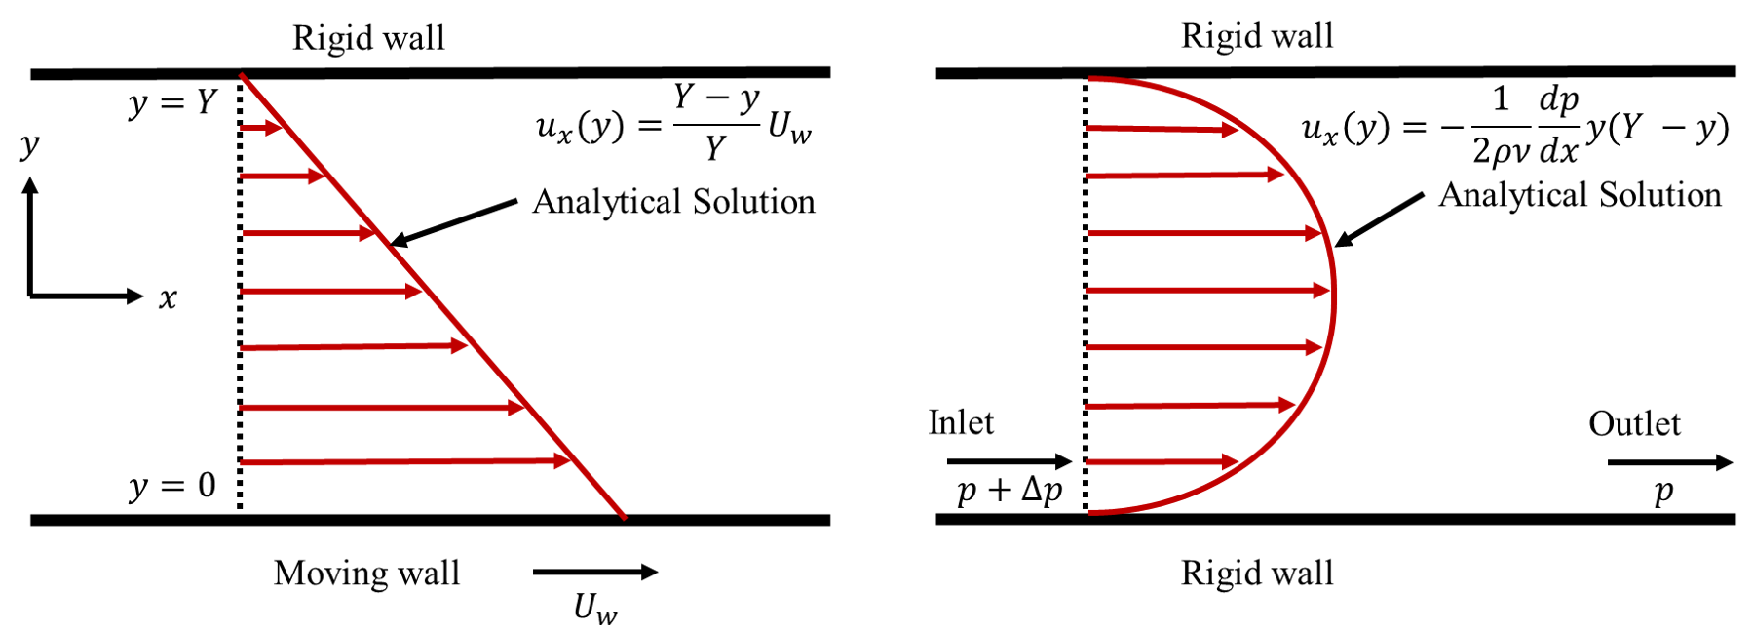
\includegraphics[width=0.98\textwidth]{imgs/couette_and_poiseuille.pdf}
  \caption{The conceptual visualizations of the Couette flow (Left) and
  Poiseuille flow (Right).}
  \vspace{-5mm}
  \label{couette-and-poiseuille-conceptual}
\end{figure}


\subsection{Couette flow}
The Couette flow is the flow between two walls as shown in
Figure~\ref{couette-and-poiseuille-conceptual}:
One is fixed and the other moves horizontally with the velocity of $U_w$.
The flow is caused by the viscous drag force acting on the fluid.
Since the Couette flow also has an analytical solution,
we can validate the implementation of the moving wall.
The analytical solution for Figure~\ref{couette-and-poiseuille-conceptual} is given by~\cite{nagy2019graphical}:
\begin{equation}
\begin{aligned}
  u_x(y) =\frac{Y - y}{Y}U_w
\end{aligned}
\end{equation}
where $Y$ is the distance between the two walls
and $u_x(y)$ is the horizontal velocity of the flow
at the location of $y$. 
In the experiment, we apply the bounce-back boundary condition
at the moving wall and the rigid wall
and the PBC at the inlet and outlet.
The results are shown in Figure~\ref{fig:couette-velocity-evolution}.
As shown in the figures, the flow velocity iteratively approaches
the analytical solution and it perfectly fits in the end
and {\bf the velocity stops growing} as seen at $t=12000 \sim 21000$.
From this experiment, the moving wall can be validated.

\begin{figure}[H]
  \vspace{-1mm}
  \centering
  \includegraphics[width=0.58\textwidth]{../log/couette_flow/fig/couette_flow_joint.pdf}
  \vspace{-5mm}
  \caption{The velocity evolution at
  $x = 25$ in the lattice grid size of $(50, 50)$.
  The wall velocity $U_w$ at the bottom and the relaxation term $\omega$ are set
  to $0.5$ and $1.20$ respectively.
  We use {\bf dry node} as described in Section~\ref{boundary-handling-section}
  and the computation of wall density follows Section~\ref{boundary-wall-settings}.
  The initial density and velocity are $\rho(\xv) = 1.0, \uv(\xv) = (0, 0)$.
  \label{fig:couette-velocity-evolution}}
\end{figure}

\subsection{Poiseuille flow}
The Poiseuille flow is the flow between two non-moving walls as shown in Figure~\ref{couette-and-poiseuille-conceptual}.
The flow is caused by a constant pressure difference $\od{p}{x}$
in the horizontal direction of the two walls.
The Poiseuille flow also has the analytical solution
and we can validate the implementation of the pressure PBC.
The analytical solution for Figure~\ref{couette-and-poiseuille-conceptual} is given by~\cite{mendiburu2009analytical}:
\begin{equation}
\begin{aligned}
  u_x(y) = - \frac{1}{2\rho \nu} \od{p}{x} y (Y - y)
\end{aligned}
\end{equation}
In the experiment, we apply the bounce-back boundary condition
at the moving wall and the rigid wall
and the pressure PBC at the inlet and outlet.
Figure~\ref{fig:poiseuille-velocity-evolution} presents the results
and the simulated results approach the analytical solutions as in the Couette flow.
In the end, it fits completely
and {\bf the velocity stops growing} as seen at $t=12000 \sim 21000$.

\begin{figure}[H]
  \centering
  \includegraphics[width=0.58\textwidth]{../log/poiseuille_flow/fig/poiseuille_flow_joint.pdf}
  \vspace{-3mm}
  \caption{The velocity evolution at
  $x = 25$ in the lattice grid size of $(50, 50)$.
  The relaxation term $\omega$ is set to $1.20$.
  The density factor at the inlet and the density factor
  at the outlet are set to $0.301$ and $0.3$ respectively.
  The initial density and velocity are $\rho(\xv) = 1.0, \uv(\xv) = (0, 0)$.
  \label{fig:poiseuille-velocity-evolution}}
\end{figure}

\section{Lid-driven cavity}
Finally, we handle a concrete example.
In this paper, the lid-driven cavity shown in Figure~\ref{lid-driven-cavity-conceptual} is simulated.
The lid-driven cavity simulates the flow inside a box with
three rigid walls and one moving wall, i.e. a lid.
In this simulation, the turbulence is caused 
when the following Reynolds number is larger than 1000~\cite{chiang1998effect}:
\begin{equation}
\begin{aligned}
  \text{Re} = \frac{LU}{\nu}
\end{aligned}
\end{equation}
where $L$ is the characteristic length parameter
of the body and $U$ is the stream flow velocity.
One key property of the Reynolds number is that two flow system
is dynamically similar if the Reynolds number and the geometry are similar~\cite{kundu2008fluid}.
Therefore, we present the results with various 
viscosity $\nu$ and the wall velocity $U = U_w$ that 
satisfy the Reynolds number of $1000$ under $L = X = Y = 300$
in Figure~\ref{fig:sliding-lid-reynolds-comparison}.
In the figures, all the settings converge to a similar flow in the end
as indicated in the key property of the Reynolds number.
Figure~\ref{fig:sliding-lid-velocity-evolution} shows the time evolution of
the streaming plot with the Reynolds number of $1000$.
The series of figure shows that the streaming changes gradually
and starts to have spirals at a corner due to the turbulence.
{\bf The time evolution of the velocity streaming plot is provided in
Github}~\footnote{https://github.com/nabenabe0928/high-performance-computing-fluid-dynamics-with-python/}.
Note that all the experiments for
Figure~\ref{fig:sliding-lid-reynolds-comparison}, \ref{fig:sliding-lid-velocity-evolution}
are {\bf performed using MPI of 9 processes}
and Table~\ref{tab:parallel-validation}
shows the validation of the parallel implementation.
Since the summation of the absolute error of the velocity over the whole domain
is $0.0$, it is obvious that
{\bf the parallel implementation behaves identically to the serial implementation}.

\begin{figure}[t]
  \vspace{-7mm}
  \centering
  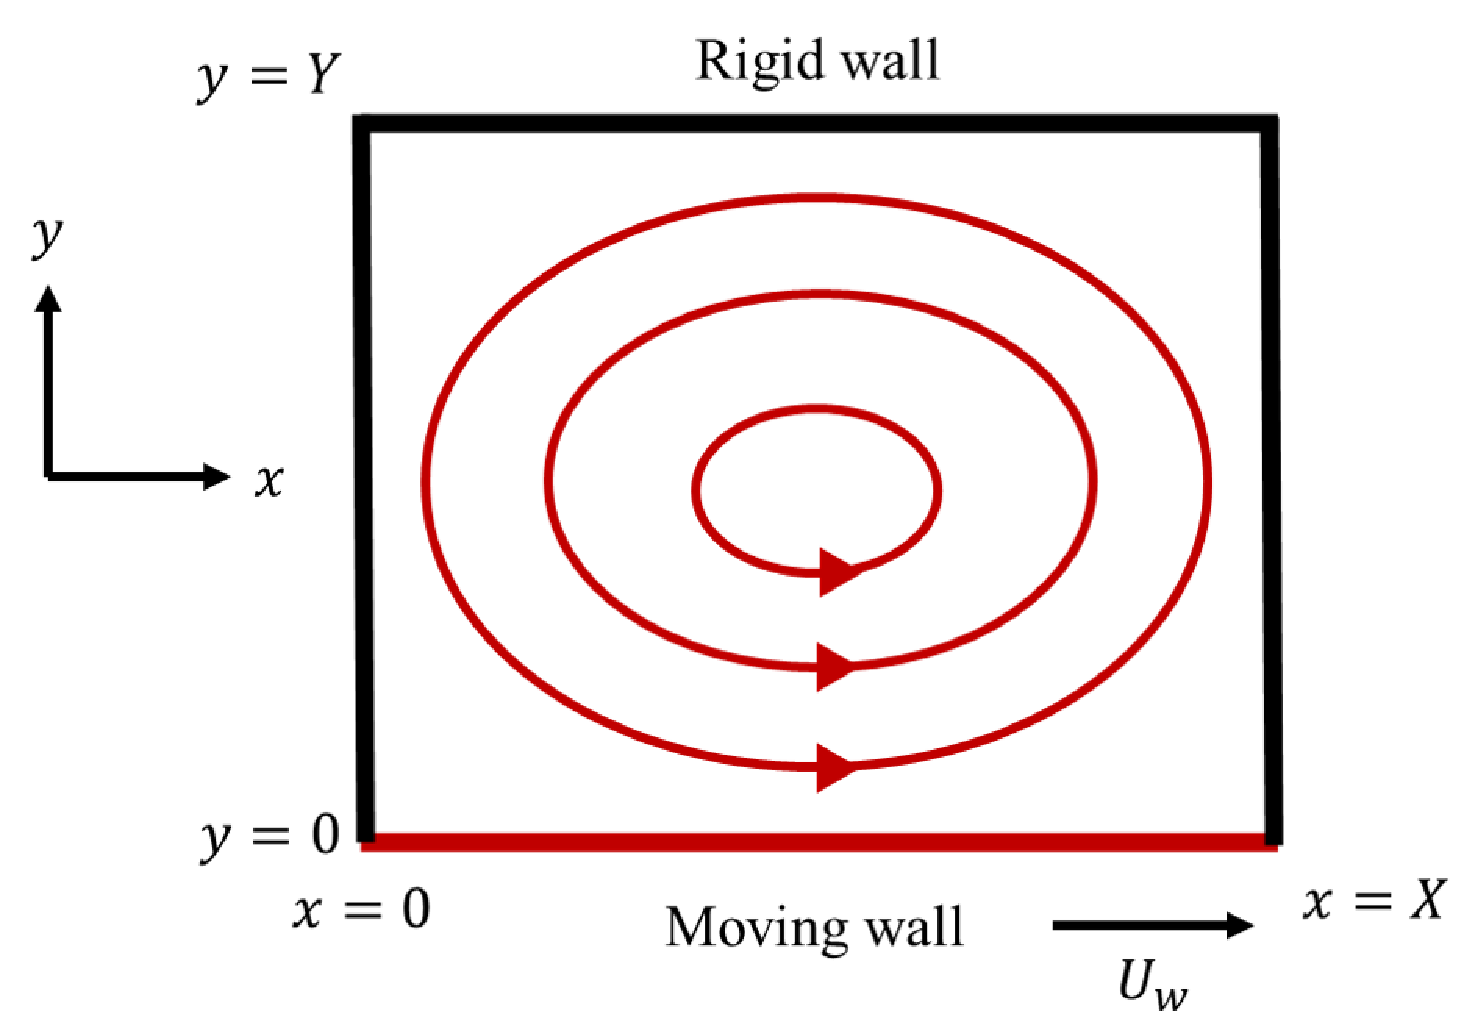
\includegraphics[width=0.48\textwidth]{imgs/lid-driven-cavity.pdf}
  \vspace{-3mm}
  \caption{The conceptual visualizations of the lid-driven cavity.}
  \label{lid-driven-cavity-conceptual}
  \vspace{-3mm}
\end{figure}

\begin{figure}[t]
  \begin{center}
    \subfloat[$U_w = 0.1, \nu = 0.03$]{
      \includegraphics[width=0.24\textwidth]{../log/sliding_lid_W0.10_visc0.03_size75x75/fig/vel_flow095000.pdf}
    }
    \subfloat[$U_w = 0.2, \nu = 0.06$]{
      \includegraphics[width=0.24\textwidth]{../log/sliding_lid_W0.20_visc0.06_size75x75/fig/vel_flow095000.pdf}
    }
    \subfloat[$U_w = 0.3, \nu = 0.09$]{
      \includegraphics[width=0.24\textwidth]{../log/sliding_lid_W0.30_visc0.09_size75x75/fig/vel_flow095000.pdf}
    }
    \subfloat[$U_w = 0.4, \nu = 0.12$]{
      \includegraphics[width=0.24\textwidth]{../log/sliding_lid_W0.40_visc0.12_size75x75/fig/vel_flow095000.pdf}
    }\\
    \subfloat[$U_w = 0.1, \nu = 0.03$]{
      \includegraphics[width=0.24\textwidth]{../log/sliding_lid_W0.10_visc0.03_size150x150/fig/vel_flow095000.pdf}
    }
    \subfloat[$U_w = 0.2, \nu = 0.06$]{
      \includegraphics[width=0.24\textwidth]{../log/sliding_lid_W0.20_visc0.06_size150x150/fig/vel_flow095000.pdf}
    }
    \subfloat[$U_w = 0.3, \nu = 0.09$]{
      \includegraphics[width=0.24\textwidth]{../log/sliding_lid_W0.30_visc0.09_size150x150/fig/vel_flow095000.pdf}
    }
    \subfloat[$U_w = 0.4, \nu = 0.12$]{
      \includegraphics[width=0.24\textwidth]{../log/sliding_lid_W0.40_visc0.12_size150x150/fig/vel_flow095000.pdf}
    }\\
    \subfloat[$U_w = 0.1, \nu = 0.03$]{
      \includegraphics[width=0.24\textwidth]{../log/sliding_lid_W0.10_visc0.03_size225x225/fig/vel_flow095000.pdf}
    }
    \subfloat[$U_w = 0.2, \nu = 0.06$]{
      \includegraphics[width=0.24\textwidth]{../log/sliding_lid_W0.20_visc0.06_size225x225/fig/vel_flow095000.pdf}
    }
    \subfloat[$U_w = 0.3, \nu = 0.09$]{
      \includegraphics[width=0.24\textwidth]{../log/sliding_lid_W0.30_visc0.09_size225x225/fig/vel_flow095000.pdf}
    }
    \subfloat[$U_w = 0.4, \nu = 0.12$]{
      \includegraphics[width=0.24\textwidth]{../log/sliding_lid_W0.40_visc0.12_size225x225/fig/vel_flow095000.pdf}
    }\\
    \subfloat[$U_w = 0.1, \nu = 0.03$]{
      \includegraphics[width=0.24\textwidth]{../log/sliding_lid_W0.10_visc0.03_size300/fig/vel_flow095000.pdf}
    }
    \subfloat[$U_w = 0.2, \nu = 0.06$]{
      \includegraphics[width=0.24\textwidth]{../log/sliding_lid_W0.20_visc0.06_size300/fig/vel_flow095000.pdf}
    }
    \subfloat[$U_w = 0.3, \nu = 0.09$]{
      \includegraphics[width=0.24\textwidth]{../log/sliding_lid_W0.30_visc0.09_size300/fig/vel_flow095000.pdf}
    }
    \subfloat[$U_w = 0.4, \nu = 0.12$]{
      \includegraphics[width=0.24\textwidth]{../log/sliding_lid_W0.40_visc0.12_size300/fig/vel_flow095000.pdf}
    }\\
    \caption{The stream plots of the lid-driven cavity
    with the lattice grid size of $(75, 75), (150, 150), (225, 225), (300, 300)$.
    (a) -- (d), (e) -- (h), (i) -- (l), (m) -- (p) are chosen to satisfy the Reynolds number
    250, 500, 750, 1000, respectively.
    We perform the update $T = 100000$ times for each setting.
    The computation of wall density follows Section~\ref{boundary-wall-settings}.
    The initial density and velocity are $\rho(\xv) = 1.0, \uv(\xv) = (0, 0)$.
      \label{fig:sliding-lid-reynolds-comparison}}
  \end{center}
\end{figure}

\begin{figure}[t]
  \begin{center}
    \subfloat[$t = 5000$]{
      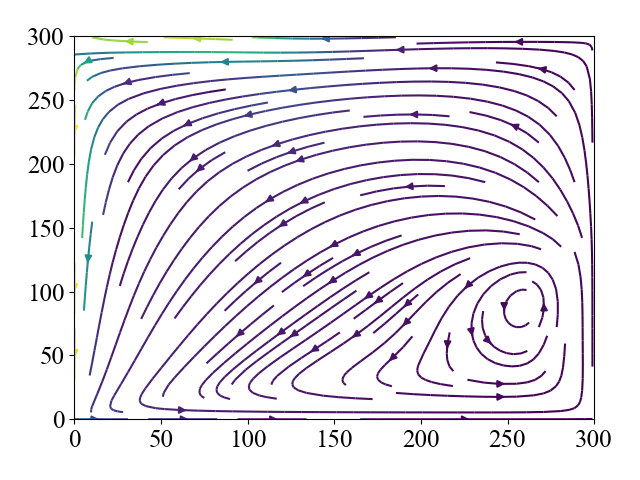
\includegraphics[width=0.30\textwidth]{../log/sliding_lid_W0.10_visc0.03_size300/fig/vel_flow005000.pdf}
    }
    \subfloat[$t = 10000$]{
      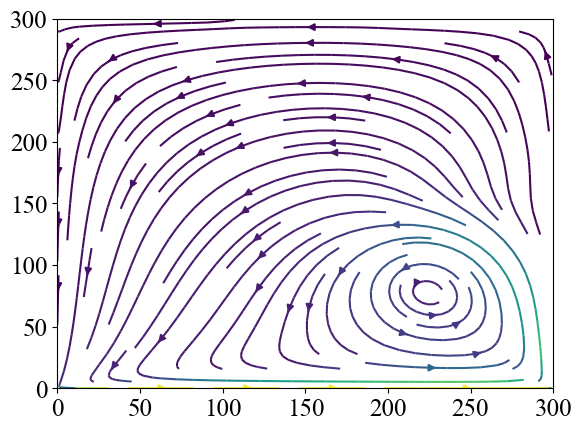
\includegraphics[width=0.30\textwidth]{../log/sliding_lid_W0.10_visc0.03_size300/fig/vel_flow010000.pdf}
    }
    \subfloat[$t = 20000$]{
      \includegraphics[width=0.30\textwidth]{../log/sliding_lid_W0.10_visc0.03_size300/fig/vel_flow020000.pdf}
    }\\
    \vspace{-3mm}
    \subfloat[$t = 30000$]{
      \includegraphics[width=0.30\textwidth]{../log/sliding_lid_W0.10_visc0.03_size300/fig/vel_flow030000.pdf}
    }
    \subfloat[$t = 50000$]{
      \includegraphics[width=0.30\textwidth]{../log/sliding_lid_W0.10_visc0.03_size300/fig/vel_flow050000.pdf}
    }
    \subfloat[$t = 100000$]{
      \includegraphics[width=0.30\textwidth]{../log/sliding_lid_W0.10_visc0.03_size300/fig/vel_flow095000.pdf}
    }\\
    \caption{
      The time evolution of the stream plots of the lid-driven cavity
    with the Reynolds number of $1000$.
    In this experiment, the lattice grid size is $(300, 300)$,
    the viscosity $\nu$ and the wall velocity are set to $0.03$ and $0.1$, respectively.
    The computation of wall density follows Section~\ref{boundary-wall-settings}.
    The initial density and velocity are $\rho(\xv) = 1.0, \uv(\xv) = (0, 0)$.
    {\bf The gif file for this experiment is available at Github} as described in footnote 3.
    }
    \label{fig:sliding-lid-velocity-evolution}
  \end{center}
\end{figure}

% \footnotetext{aaaaa}

\begin{table}
  \begin{center}
    \caption{The validation of the parallel implementation by comparing
    the velocity field in the serial and the parallel implementations.
    The parallel implementation is performed by the number of processes $P = 9$.
    We set the lattice grid size is $(X, Y) = (30, 30)$,
    the wall velocity $U_w = 0.1$ and the viscosity $\nu = 0.03$
    and perform $T = 10000$ updates.
    The initial density and velocity are $\rho(\xv) = 1.0, \uv(\xv) = (0, 0)$.
    }
    \vspace{2mm}
    \label{tab:parallel-validation}
    \begin{tabular}{llll}
      \toprule
       & Max & Min & Sum of absolute values \\
      \midrule
      Velocity $\uv_p$ in parallel implementation & -0.03711 & 0.09372 & 32.06084 \\
      Velocity $\uv_s$ in serial implementation & -0.03711 & 0.09372 & 32.06084 \\
      The absolute difference $|| \uv_p - \uv_s ||$ & {\bf 0.0} & {\bf 0.0} & {\bf 0.0} \\
      \bottomrule
    \end{tabular}
  \end{center}
  \vspace{-5mm}
\end{table}

This experiment requires a long time to complete.
For example, it takes 1 hour to finish one simulation using
intel core i7--10700 and 32GB RAM.
Recall that the advantage of the LBM is to allow us to compute the simulation in
parallel easily.
For this reason, we test the scalability of this simulation using
various numbers of processes.
Note that all the experiments related to the scaling test
are performed on {\bf BWUniCluster}
\footnote{https://wiki.bwhpc.de/e/Category:BwUniCluster\_2.0}.
The implementation follows Section~\ref{section-mpi}
and each thread is bound to one processor.
Figure~\ref{fig:sliding-lid-scaling} shows the plot of
MLUPS, a.k.a. million lattice updates per second, and
the number of processes.
As seen in the figure, the larger grid size leads to
less MLUPS with the smaller number of processes.
This is due to the heavy load on small number of processors.
On the other hand, as the number of processes
becomes larger, the simulation with a larger domain exhibits
higher efficiency.
Ideally, the MLUPS should grow linearly with respect to the number of processes.
However, it does not happen because of the latency of the communication
and the waiting for the synchronization as described in Amdahl's law~\cite{amdahl1967validity}.
It explains why the larger domain leads to more scalability with respect to
the number of processes.


\begin{figure}[b]
  \centering
  \includegraphics[width=0.88\textwidth]{../log/scaling_test.pdf}
  \vspace{-3mm}
  \caption{The scaling test of the lid-driven cavity simulation.
  The grid size is either $100 \times 100, 300 \times 300 \text{ or } 1000 \times 1000$.
  The number of processes are $1 ,4 ,9 ,16 ,25 ,36 ,100 ,144 ,225 ,400$ respectively.
  Note that both axes are log-scale.
    The viscosity and the wall velocity are set to $\nu = 0.03$ and $0.1$
    and we perform the update $T = 10000$ times.
    The initial density and velocity are $\rho(\xv) = 1.0, \uv(\xv) = (0, 0)$.
  }
  \label{fig:sliding-lid-scaling}
\end{figure}
